\chapter{参数方程、极坐标}
\section{参数方程}
\subsection{曲线的参数方程}
前面我们所研究过的曲线方程 $F\,(x,y) = 0$,都是表示曲线上任意一点 $x$、$y$ 之间的直接关系的。
但是在解决某些问题时,对于曲线上任意点,它们的坐标 $x$、$y$ 的这种关系往往不容易发现,而通过另一个变数间接地表示 $x$、$y$ 之间的关系却比较方便。
下面我们看一个例子。

设炮弹的发射角为 $\alpha$,发射的初速度为 $v_0$,求弹道曲线的方程(不计空气阻力)。

弹道曲线是炮弹飞行的轨迹。
它上面的各个点都表示炮弹发射后某个时刻的位置。
当这个时刻确定后,炮弹的位置就确定了。

\medskip\noindent
\begin{minipage}{0.55\linewidth}\parindent2em
取炮口为原点,水平方向为 $x$ 轴,建立直角坐标系(\cref{fig:4-1})。设炮弹发射后的位置在点 $M\,(x,y)$,因为炮弹在 $Ox$ 方向是以 $v_0\cos\alpha$ 为速度的匀速直线运动,在 $Oy$ 方向是以 $v_0\sin\alpha$ 为初速度的竖直上抛运动。按匀速直线运动和竖直上抛运动的位移公式,得
\end{minipage}\hfill
\begin{minipage}{0.4\linewidth}\centering
  \begin{figurehere}
    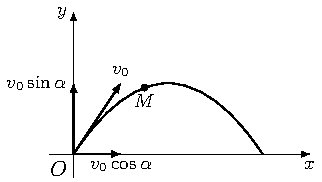
\includegraphics{4-1.pdf}
    \caption{}\label{fig:4-1}
  \end{figurehere}
\end{minipage}
\begin{equation}
  \label{eq:trajectory}
  \begin{cases}
    x=v_0\cos\alpha\cdot t,\\
    y=v_0\sin\alpha\cdot t-\dfrac{1}{2}gt^2,
  \end{cases}
\end{equation}
$g$ 是重力加速度(取 \qty{9.8}{m/s^2})。



这里,$v_0$、$\alpha$ 和 $g$ 都是常数,当 $t$ 取某一个允许值时,由方程组~\eqref{eq:trajectory} 就可以确定当时炮弹所在的位置。这就是说,当 $t$ 确定时,点 $M\,(x,y)$ 的位置也就随着确定了。这样建立 $t$ 与 $x$、$y$ 之间的关系不仅方便,而且还可以反映变数的实际意义。如方程组~\eqref{eq:trajectory} 中的两个方程就分别反映出炮弹飞行的水平距离、高度与时间的关系。

一般地,在取定的坐标系中,如果曲线上任意一点的坐标 $x$、$y$ 都是某个变数 $t$ 的函数
\begin{equation}
  \label{eq:parameter_function}
  \begin{cases}
    x=f(t),\\
    y=\varphi(t),
  \end{cases}
\end{equation}
并且对于 $t$ 的每一个允许值,由方程组 \eqref{eq:parameter_function} 所确定的点 $M\,(x,y)$ 都在这条曲线上,那么方程组 \eqref{eq:parameter_function} 就叫做这条曲线的\Concept{参数方程},联系 $x$、$y$ 之间关系的变数叫做\Concept{参变数},简称\Concept{参数}。参数方程中的参数可以是有物理、几何意义的变数,也可以是没有明显意义的变数。

相对于参数方程来说,前面学过的直接给出曲线上点的坐标关系的方程,叫做曲线的\Concept{普通方程}。
\begin{example}
  如\cref{fig:4-2},以原点为圆心,分别以 $a$、$b$($a>b$)为半径作两个圆。点 $B$ 是大圆半径与小圆的交点,过点 $A$ 作 $AN\perp Ox$,垂足为 $N$,过点 $B$ 作 $BM \perp AN$,垂足为 $M$。求当半径 $OA$ 绕点 $O$ 旋转时,点 $M$ 的轨迹的参数方程。
\end{example}

\noindent
\begin{minipage}{0.6\linewidth}\parindent2em
\begin{solution}
  设点 $M$ 的坐标是 $(x,y)$,$\phi$ 是以 $Ox$ 为始边,$OA$ 为终边的正角。取 $\phi$ 为参数,那么
  \begin{align*}
    x&=ON=|OA|\cos\phi,\\
    y&=NM=|OB|\sin\phi.
  \end{align*}
  也就是
  \[\begin{cases}x=a\cos\phi,\\y=b\sin\phi.\end{cases}\]
\end{solution}
\end{minipage}\hfill
\begin{minipage}{0.35\linewidth}\centering
  \begin{figurehere}
    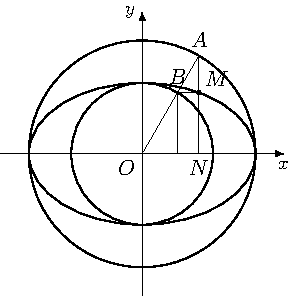
\includegraphics{4-2.pdf}
    \caption{}\label{fig:4-2}
  \end{figurehere}
\end{minipage}

\medskip\noindent
这就是所求点 $M$ 的轨迹的参数方程(图形是一个椭圆)。

\begin{example}
  求经过点 $M_0\,(x_0,y_0)$,倾斜角为 $\alpha$ 的直线 $l$ 的参数方程。
\end{example}
\begin{solution}
  设点 $M_0\,(x,y)$ 是直线上任意一点,过点 $M$ 作 $y$ 轴的平行线,过点 $M_0$ 作 $x$ 轴的平行线,两直线相交于点 $Q$。规定直线 $l$ 向上的方向为正方向(\cref{fig:4-3})。

当 $\overline{M_0M}$ 与 $l$ 同方向,或两点 $M$、$M_0$ 重合时,因 $M_0M=|M_0M|$,由三角函数定义,有
\[M_0Q=M_0M\sin\alpha,\quad QM=M_0M\sin\alpha.\]

当 $\overline{M_0M}$ 与 $l$ 反方向时,$M_0M$、$M_0Q$、$QM$ 同时改变符号,上式仍然成立。
\end{solution}

\medskip\noindent
\begin{minipage}{0.6\linewidth}\parindent2em
  设 $M_0M=t$,取 $t$ 为参数。
  \begin{gather*}
    \because\quad M_0Q=x-x_0,\\
    QM=y-y_0,\\
    \therefore \quad x-x_0=t\cos\alpha,\\
     y-y_0=t\sin\alpha,\\
  \end{gather*}
\end{minipage}\hfill
\begin{minipage}{0.35\linewidth}\centering
\begin{figurehere}
  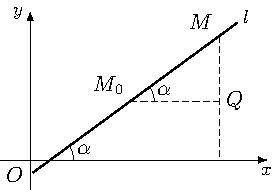
\includegraphics{4-3.pdf}
  \caption{}\label{fig:4-3}  
\end{figurehere}
\end{minipage}

\medskip\noindent
即
\[\begin{cases}x=x_0+t\cos\theta,\\y=y_0+t\sin\theta.\end{cases}\]
这就是所求直线 $l$ 的参数方程。

\begin{Practice}
  \begin{question}
    \item\label{prac:4-1-1} 求半径为 $r$ 、圆心在原点 $O$ 的圆的参数方程。(提示:以 $\phi$ 为参数,如图。)
    \begin{figurehere}
      \begin{minipage}{\linewidth}\centering
        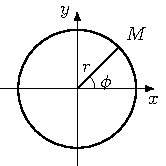
\includegraphics{pr4-1-1.pdf}
        \caption*{(第 \ref{prac:4-1-1} 题)}
      \end{minipage}
    \end{figurehere}
    \item 已知一条直线上两点 $M_1\,(x_1,y_1)$、$M_2\,(x_2,y_2)$,以分点 $M\,(x,y)$ 分 $\overline{M_1M_2}$ 所成的比 $\lambda$ 为参数,写出参数方程。
  \end{question}
\end{Practice}

\subsection{参数方程和普通方程的互化}
参数方程和普通方程是曲线方程的不同形式,它们都是表示曲线上点的坐标之间关系的。
一般情况下,我们可以通过消去参数方程中参数,得出直接表示 $x$、$y$ 之间关系的普通方程;也可以选择一个参数将普通方程变成参数方程的形式,如果参数选择得适当,方程可能比较简单或者较明显地反映出物理、几何意义。

\begin{example}
  把弹道曲线的参数方程
  \begin{numcases}{}
    \label{eq:x_trace} x=v_0t\cos\alpha,\\
    \label{eq:y_trace} y=v_0t\sin\alpha-\frac{1}{2}gt^2
  \end{numcases}
  化为普通方程,并求出炮弹水平射程的公式。
\end{example}
\begin{solution}
  由 \eqref{eq:x_trace} 得
  \[t=\frac{x}{v_0\cos\alpha}.\]

  代入\eqref{eq:y_trace},消去参数 $t$,得普通方程
  \[ y=-\frac{g}{2v_0^2\cos^2\alpha}x^2+\frac{\sin\alpha}{\cos\alpha}x.\]
  这是抛物线方程。

  在这个方程里,令 $y=0$,得 $x_1=0$,$x_2=\dfrac{v_0^2\sin2\alpha}{g}$。炮弹的水平射程公式为
  \[s=x_2-x_1=\frac{v_0^2\sin2\alpha}{g}.\]
\end{solution}

\begin{example}
  把参数方程
  \[\begin{cases}x=a\cos\phi,\\y=b\sin\phi,\end{cases}\quad(a>b>0)\]
  化为普通方程。
\end{example}
\begin{solution}
  分别将两方程变形得
  \[\begin{cases}\dfrac{x}{a}=\cos\phi,\\\dfrac{y}{b}=\sin\phi.\end{cases}\]
  再将两方程的两边平方后相加,得
  \[\frac{x^2}{a^2}+\frac{y^2}{b^2}=\cos^2\phi+\sin^2\phi,\]
  即
  \[\frac{x^2}{a^2}+\frac{y^2}{b^2}=1.\]
  这是中心在原点,焦点在 $x$ 轴上的椭圆方程。
\end{solution}

\begin{example}
  化直线的点斜式方程 $y-y_0=\tan\alpha(x-x_0)$ 为参数方程。
\end{example}
\begin{solution}
  将直线的点斜式方程变形为
  \[\frac{y-y_0}{\sin\alpha}=\frac{x-x_0}{\cos\alpha}.\]
  设上述比值为 $t$,取 $t$ 为参数,得
  \[\begin{cases}\dfrac{x-x_0}{\cos\alpha},\\\dfrac{y-y_0}{\sin\alpha}.\end{cases}\]
  即
  \[\begin{cases} x=x_0+t\cos\alpha, \\[10pt] y=y_0+t\sin\alpha .\end{cases}\]
  这就是经过点 $P_0\,(x_0,y_0)$,倾斜角为 $\alpha$ 的直线的参数方程。
\end{solution}

\begin{Practice}
  \begin{question}
    \item 把下列参数方程($\phi$、$t$ 是参数)化成普通方程,并说明它们各表示什么曲线:
    \begin{tasks}(2)
      \task $\begin{cases}x=\cos\phi,\\y=\sin\phi; \end{cases}$
      \task $\begin{cases}x=2pt^2,\\y=2pt; \end{cases}(p>0)$
      \task $\begin{cases}x=x_1+at,\\y=y_1+bt. \end{cases}$
    \end{tasks}
    \item 根据所给条件,把下列各方程化成参数方程:
    \begin{tasks}
      \task $xy=a^2$,设 $x=a\tan\phi$,$\phi$ 是参数;
      \task $\dfrac{x^2}{a^2}-\dfrac{y^2}{b^2}=1$,设 $y=b\tan\phi$,$\phi$ 是参数。
    \end{tasks}
  \end{question}
\end{Practice}

\subsection{圆的渐开线、摆线}
\medskip\noindent
\begin{minipage}{0.5\linewidth}\parindent2em
一些机器零件常用某些特殊曲线作外形线。
例如,大多数齿轮都采用渐开线齿形(\cref{fig:4-4}),也有采用摆线齿形或其他齿形的。
用渐开线齿形或摆线齿形的齿轮磨损少,传动平稳,具有省力、耐用和噪音小的特点。
这两种曲线用参数方程来表示比较方便。
下面我们来求这两种曲线的参数方程。
\end{minipage}\hfill
\begin{minipage}{0.45\linewidth}\centering
\begin{figurehere}
  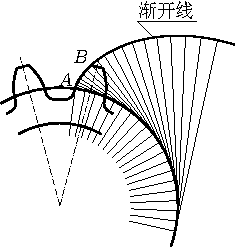
\includegraphics{4-4.pdf}
  \caption{}\label{fig:4-4}
\end{figurehere}
\end{minipage}

\subsubsection{圆的渐开线}
如\cref{fig:4-5},把一条没有弹性的细绳绕在一个固定的圆盘的侧面上,将铅笔系在绳的外端,把绳拉紧逐渐地展开(这时绳的拉直部分和圆保持相切),铅笔所画出的曲线,即绳的外端的轨迹叫做\Concept{圆的渐开线}。这个圆叫做渐开线的\Concept{基圆}。
\begin{figure}
  \begin{minipage}[b]{0.48\linewidth}\centering
    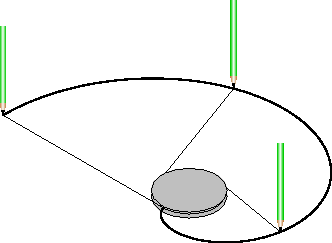
\includegraphics{4-5.pdf}
    \caption{}\label{fig:4-5}
  \end{minipage}
  \begin{minipage}[b]{0.48\linewidth}\centering
    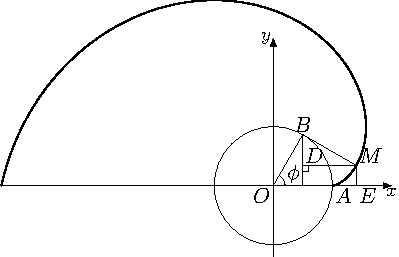
\includegraphics{4-6.pdf}
    \caption{}\label{fig:4-6}
  \end{minipage}
\end{figure}

下面我们来推导圆的渐开线的参数方程。

设基圆的圆心为 $O$,半径为 $r$,细绳外端的初始位置为 $A$。以 $O$ 为原点,有向直线 $OA$ 为 $x$ 轴,建立直角坐标系(\cref{fig:4-6})。

设点 $M\,(x,y)$ 是圆的渐开线上任意一点,$BM$ 是圆的切线,$B$ 为切点,连结 $OB$,$\angle AOB= \phi$ (弧度)是以 $OA$ 为始边,$OB$ 为终边的正角。取 $\phi$ 为参数,根据圆的渐开线的定义,切线 $BM$ 的长等于 $\overparen{AB}$ 的长 $r\phi$。

作 $ME\perp Ox$,$BC\perp Ox$,$MD\perp BC$,垂足分别为 $E$、$C$、$D$,则 $\angle MBD=\phi$。由此可得点 $M$ 的坐标:
\begin{align*}
  x&=OE=OC+CE=OC+DM\\
  &=|OB|\cos\phi+|BM|\sin\phi\\
  &=r\cos\phi+r\phi\sin\phi,\\
  y&=EM=CD=CB-BD\\
  &=|OB|\sin\phi-|BM|\cos\phi\\
  &=r\sin\phi-r\phi\cos\phi.
\end{align*}

因此,所求圆的渐开线的参数方程是
\[\begin{cases}x=r(\cos\phi+\phi\sin\phi),\\y==r(\sin\phi-\phi\cos\phi).\end{cases}\]

\begin{Practice}\noindent
  \begin{minipage}{0.36\linewidth}
  \begin{question}
    \item 将圆的渐开线中的基圆换为正方形就得到正方形的渐开线。用刻度尺、圆规画出边长为 \qty{1}{cm} 的正方形的渐开线。
    \item \label{prac:4-3-2}如图,有一标准的渐开线齿轮,齿轮的齿廓线的基圆直径是 \qty{225}{mm},求齿廓线 $AB$ 所在渐开线的参数方程。
  \end{question}
\end{minipage}\hfill
\begin{minipage}{0.59\linewidth}\centering
  \begin{figurehere}
    \begin{minipage}{\linewidth}\centering
      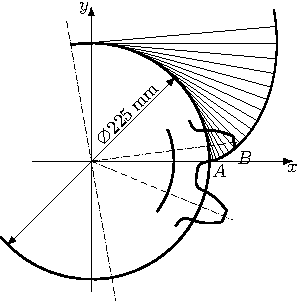
\includegraphics{pr4-3-2.pdf}
      \caption*{(第 \ref{prac:4-3-2} 题)}
    \end{minipage}
  \end{figurehere}
\end{minipage}
\end{Practice}

\subsubsection{摆线}
一个圆沿着一条定直线滚动时,圆周上的一个定点 $M$ 的轨迹叫做摆线,又叫旋轮线(\cref{fig:4-7})。
\begin{figure}
  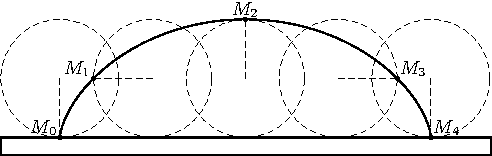
\includegraphics{4-7.pdf}
  \caption{}\label{fig:4-7}  
\end{figure}

下面我们求摆线的参数方程。

设圆的半径为 $a$,取圆滚动所沿的直线为 $x$ 轴,圆上定点 $M$ 落在直线上的一个位置为原点,建立直角坐标系(\cref{fig:4-8})。圆滚动 $\phi$ 角后圆心在点 $B$,并与 $x$ 轴相切于点 $A$。作 $MD\perp Ox$,$MC\perp BA$,垂足分别为 $D$、$C$。用 $(x,y)$ 表示点 $M$ 的坐标,取 $\phi$ 作参数,那么,$OA$ 的长等于 $\overparen{MA}$ 的长,得
\begin{align*}
  x&=OD=OA-DA=a\phi-a\sin\phi,\\
  y&=DM=AC=AB-CB=a-a\cos\phi.
\end{align*}

\begin{figure}
  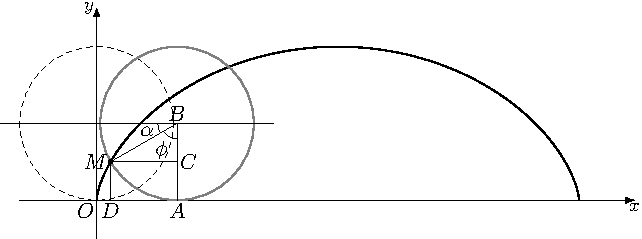
\includegraphics{4-8.pdf}
  \caption{}\label{fig:4-8}  
\end{figure}

因此,所求摆线的参数方程是
\[ \begin{cases}x=a(\phi-\sin\phi),\\y=a(1-\cos\phi).\end{cases} \]

当圆滚动一周,即 $\phi$ 由 0 变到 $2\uppi$ 时,点 $M$ 描出摆线的第一拱。
圆向前再滚动一周,$\phi$ 从 $2\uppi$ 变到 $4\uppi$,点 $M$ 描出摆线的第二拱。
显然,第二拱的形状和第一拱完全相同。
圆继续向前滚动,可得第三拱、第四拱、……。
圆向后滚动的情况也一样。
可见摆线是无数段拱形弧组成的,拱宽为 $2\uppi a$,拱高为 $2a$。

摆线有一些重要的性质,例如,物体在重力作用下从点 $A$ 滑落到点 $B$(无摩擦),物体滑落所需时间最短的路线,不是沿点 $A$ 到点 $B$ 的直线,而是沿从 $A$ 到 $B$ 的一段摆线,如\cref{fig:4-9}。
因此摆线又叫最速降线。
\begin{figure}
  \begin{minipage}[b]{0.65\linewidth}\centering
    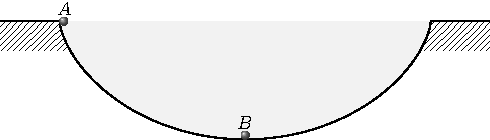
\includegraphics{4-9.pdf}
    \caption{}\label{fig:4-9}  
  \end{minipage}
  \begin{minipage}[b]{0.3\linewidth}\centering
    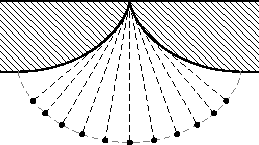
\includegraphics{4-10.pdf}
    \caption{}\label{fig:4-10}  
  \end{minipage}
\end{figure}

又如普通单摆的周期与振幅的大小有关。
如果在摆的摆动平面内做两个如\cref{fig:4-10} 那样的摆线形挡板;在挡板的限制下,单摆的周期就与振幅的大小无关了,这时摆的运动轨迹也是一段摆线。
摆线的名称就是由这个性质得到的。

\begin{Practice}
  \begin{question}
    \item 求摆线
    \[\begin{cases}x=\phi-\sin\phi,\\y=1-\cos\phi\end{cases}\]
    上 $2\uppi \leqslant \phi \leqslant 4\uppi$ 这一段与直线 $y=\dfrac{3}{2}$ 的交点的坐标。\par\smallskip
    \item 有一轮子,沿着直线轨道滚动,轮子的半径是 $a$,在轮辐上有一点 $M$,与轮子中心的距离是 $b$($b<a$)。点 $M$ 的轨迹叫短摆线,求它的参数方程。
  \end{question}
\end{Practice}
\begin{Exercise}
  \begin{question}
    \item 已知弹道曲线的参数方程为
    \[\begin{cases}x=v_0t\cos\alpha,\\y=v_0t\sin\alpha-\dfrac{1}{2}gt^2.\end{cases}\]
    \begin{tasks}
      \task 求发射角 $\alpha = \dfrac{\uppi}{3}$ 时,弹道曲线的普通方程和射程;
      \task 设 $v_0$ 是定值,$\alpha$ 可以变动。求证: 当 $\alpha=\dfrac{\uppi}{4}$ 时射程最大。
    \end{tasks}
    \item 把下列参数方程化成普通方程(其中 $t$、$\phi$ 是参数),并说明各表示什么曲线:
    \begin{tasks}(2)
      \task $\begin{cases}x=3-2t,\\y=1-4t;\end{cases}$
      \task $\begin{cases}x=4\cos\phi,\\y=3\sin\phi;\end{cases}$
      \task $\begin{cases}x=\dfrac{a}{2}\left(t+\dfrac{1}{t}\right),\\y=\dfrac{b}{2}\left(t-\dfrac{1}{t}\right).\end{cases}$
    \end{tasks}
    \item 根据所给的条件,化下列方程成参数方程($t$、$\phi$ 是参数):
    \begin{tasks}
      \task $y^2=4x^2-5x^3$,$y=tx$;
      \task $4x^2+y^2-16x+12=0$,$y=2\sin\phi$。
    \end{tasks}
    \item 设 $x=2\cos\phi$,$\phi$ 是参数,求椭圆 $4x^2+y^2=16$ 的参数方程。
    \item 动点 $M$ 作等速直线运动,它在 $x$ 轴和 $y$ 轴方向的分速度分别为 9 和 12,运动开始时,点 $M$ 位于 $A\,(1,1)$,求点 $M$ 的轨迹的参数方程。
    \item 解答:
    \begin{tasks}
      \task 写出经过点 $M\,(1,5)$,倾斜角是 $\dfrac{\uppi}{3}$ 的直线的参数方程。
      \task 利用这个参数方程,求这条直线和直线 $x-y-2\sqrt{3}=0$ 的交点到点 $M$ 的距离;
      \task 求这条直线和圆 $x^2+y^2=16$ 的两个交点到点 $M$ 的距离的和与积。
    \end{tasks}
    \item\label{exec:13-7} 椭圆规是用来画椭圆的一种器械,它的构造如图所示。在一个十字形的金属板上有两条互相垂直的槽,在直尺上有两个固定滑块 $A$、$B$,它们可分别在纵槽和横槽中滑动,在直尺上的点 $M$ 用套管装上铅笔;使直尺转动一周就画出一个椭圆。说明椭圆规构造的原理。
    \begin{figurehere}
      \begin{minipage}{\linewidth}\centering
        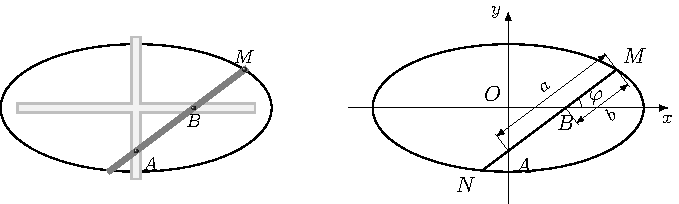
\includegraphics{ex13-7.pdf}
        \caption*{(第 \ref{exec:13-7} 题)}
      \end{minipage}
    \end{figurehere}
    (提示;可以用直尺 $AB$ 和横槽所成的角为参数,求出点 $M$ 轨迹的参数方程。)
    \item 一颗人造地球卫星的运行轨道是一个椭圆,长轴长为 \qty{15565}{km},短轴长为 \qty{15443}{km},取椭圆中心为坐标原点,求卫星轨道的参数方程。
    \item 解答:
    \begin{enumerate}[itemindent=2em]
      \item 物体从高处以初速 $v_0$\,\unit{m/s} 沿水平方向抛出。以抛出点为原点,过抛出点的水平直线为 $x$ 轴,写出物体所经路线的参数方程。
      \item 作水平飞行的飞机的速度 $v=\qty{150}{m/s}$,若在飞行高度 $H=\qty{600}{m}$ 时投弹,求
      \begin{tasks}
        \task 炸弹离开飞机后的轨迹方程;
        \task 飞机在离目标多远 (水平距离) 的地方投弹才能命中目标?
      \end{tasks}
    \end{enumerate}
    \item 一个圆沿一条直线滚动时,点 $M$ 是圆的一条半径延长线上的一点。求点 $M$ 的轨迹的参数方程。
  \end{question}
\end{Exercise}

\section{极坐标}
\subsection{极坐标系}
前面我们所使用的平面坐标系是直角坐标系,它是最简单和最常用的一种坐标系,但不是唯一的坐标系。
有时利用别的坐标系比较方便。
例如,炮兵射击时是以大炮为基点,利用目标的方位角及目标与大炮的距离来确定目标的位置的。
在航空、航海中也常使用类似的方法。
下面研究如何利用角和距离来建立坐标系。

\medskip\noindent
\begin{minipage}{0.75\linewidth}\parindent2em
在平面内取一个定点 $O$,叫做极点,引一条射线 $Ox$,叫做极轴,再选定一个长度单位和角度的正方向(通常取逆时针方向)(\cref{fig:4-11})。对于平面内任意一点 $M$,用 $\rho$ 表示线段 $OM$ 的长度,$\theta$ 表示从 $Ox$ 到 $OM$ 的角度,$\rho$ 叫做点 $M$ 的\Concept{极径},$\theta$ 叫做点 $M$ 的\Concept{极角},有序数对 $(\rho,\theta)$ 就叫做点 $M$ 的\Concept{极坐标}。
这样建立的坐标系叫做\Concept{极坐标系}。
极坐标为 $\rho$,$\theta$ 的点 $M$,可表示为 $M\,(\rho,\theta)$。
\end{minipage}\hfill
\begin{minipage}{0.2\linewidth}\centering
\begin{figurehere}
  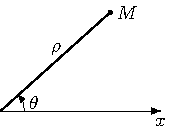
\includegraphics{4-11.pdf}
  \caption{}\label{fig:4-11}
\end{figurehere}
\end{minipage}

\medskip
当点 $M$ 在极点时,它的极坐标 $\rho=0$,$\theta$ 可以取任意值。


\medskip\noindent
\begin{minipage}{0.45\linewidth}\parindent2em
如\cref{fig:4-12},在极坐标系中,$A$、$B$、$C$、$D$、$E$、$F$、$G$ 各点的极坐标分别是 $(4,0)$、$\left(2,\dfrac{\uppi}{4}\right)$、$\left(3,\dfrac{\uppi}{2}\right)$、$\left(1,\dfrac{5\uppi}{6}\right)$、$(3.5,\uppi)$、$\left(6,\dfrac{4\uppi}{3}\right)$、$\left(5,\dfrac{5\uppi}{3}\right)$。
角也可以取负值,例如点 $B$、$D$、$F$ 的坐标也可以写作 $\left(2,-\dfrac{7\uppi}{4}\right)$、$\left(1,-\dfrac{7\uppi}{6}\right)$、$\left(6,-\dfrac{2\uppi}{3}\right)$。

\smallskip
在一般情况下,极径都是取正值。但是在某些必要的情况下,也允许取负值。
\end{minipage}\hfill
\begin{minipage}{0.5\linewidth}\centering
  \begin{figurehere}
    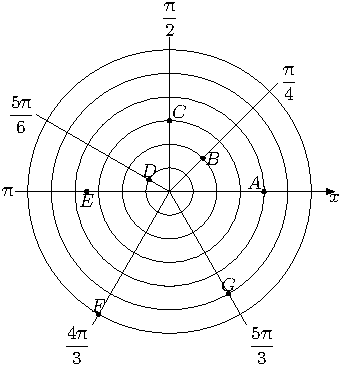
\includegraphics{4-12.pdf}
    \caption{}\label{fig:4-12}
  \end{figurehere}
\end{minipage}

\smallskip\noindent
\begin{minipage}{0.45\linewidth}\parindent2em
当 $\rho<0$ 时,点 $M\,(\rho,\theta)$ 的位置可以按下列规则确定:作射线 $OP$,使 $\angle xOP=\theta$,在 $OP$ 的反向延长线上取一点 $M$,使 $|OM|=|\rho|$。点 $M$ 就是坐标为 $(\rho,\theta)$ 的点(\cref{fig:4-13})。
\end{minipage}\hfill
\begin{minipage}{0.5\linewidth}\centering
\begin{figurehere}
  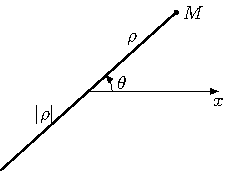
\includegraphics{4-13.pdf}
  \caption{}\label{fig:4-13}
\end{figurehere}
\end{minipage}

\smallskip\noindent
\begin{minipage}{0.45\linewidth}\parindent2em
例如\cref{fig:4-14} 中,当极径取作负值时,点 $A$、$B$、$C$、$D$、$E$ 的坐标写作 $\left(-3,\dfrac{\uppi}{6}\right)$、$\left(-4,\dfrac{11\uppi}{12}\right)$、$\left(-5,-\dfrac{\uppi}{2}\right)$、$\left(-2,-\dfrac{\uppi}{12}\right)$、$\left(-1,\dfrac{5\uppi}{4}\right)$。

\smallskip
建立极坐标系后,给定 $\rho$ 和 $\theta$,就可以在平面内确定唯一点 $M$;反过来,给定平面内一点,也可以找到它的极坐标 $(\rho,\theta)$。
但和直角坐标系不同的是,平面内一个点的极坐标可以有无数种表示法。这是因为 $(\rho,\theta)$ 和 $(-\rho,\theta+\uppi)$ 是同一点的坐标,而且一个角加 $2n\uppi$($n$ 是任意整数)后都是
\end{minipage}\hfill
\begin{minipage}{0.5\linewidth}
\begin{figurehere}
  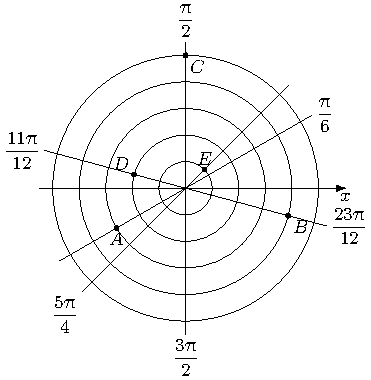
\includegraphics{4-14.pdf}
  \caption{}\label{fig:4-14}
\end{figurehere}
\end{minipage}

\medskip\noindent
和原角终边相同的角。
比如,$\left(6,\dfrac{\uppi}{6}\right)$、$\left(-6,\dfrac{\uppi}{6}+\uppi\right)$ 以及 $\left(6,\dfrac{\uppi}{6}+{2\uppi}\right)$、$\left(6,\dfrac{\uppi}{6}-2\uppi\right)$、 $\left(-6,\dfrac{\uppi}{6}+3\uppi\right)$、$\left(-6,\dfrac{\uppi}{6}-\uppi\right)$ 等等,都是同一点的极坐标。

\smallskip
一般地,如果 $(\rho,\theta)$ 是一个点的极坐标,那么 $\left(\rho,\theta+2n\uppi\right)$、$\left[-\rho,\theta+\left(2n+1\right)\uppi\right]$ 都可以作为它的极坐标(这里 $n$ 是任意整数)。
但如果限定 $\rho>0$,$0\leqslant\theta<2\uppi$ 或 $-\uppi<\theta\leqslant\uppi$,那么除极点外,平面内的点和极坐标就可以一一对应了。以下,在不作特殊说明时,认为 $\rho\geqslant 0$。

\begin{Practice}
  \begin{question}
    \item\label{prac:4-5-1} 写出图中 $A$、$B$、$C$、$D$、$E$、$F$、$G$ 各点的极坐标($\rho>0,0 \leqslant\theta<2\uppi$)。
    \begin{figurehere}
      \begin{minipage}{\linewidth}\centering
        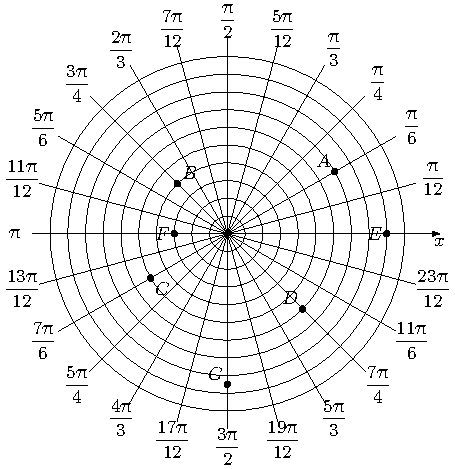
\includegraphics{pr4-5-1.pdf}
        \caption*{(第 \ref{prac:4-5-1} 题)}
      \end{minipage}
    \end{figurehere}
    \item 在极坐标系中,作出下列各点:
    \begin{tasks}
      \task $A\,\left(2,\dfrac{\uppi}{6}\right)$、$B\,(6,-\ang{120})$、$C\,\left(1,\dfrac{\uppi}{3}\right)$、$D\,\left(4,-\dfrac{3\uppi}{4}\right)$、$E\,(4,0)$、$F\,(2.5,\ang{180})$
      \task $A\,\left(3,\dfrac{\uppi}{3}\right)$、$B\,\left(3,\dfrac{\uppi}{6}\right)$、$C\,\left(3,\dfrac{\uppi}{2}\right)$、$D\,(3,\uppi)$、$E\,\left(3,\dfrac{3\uppi}{2}\right)$,并说明这五个点有什么关系;
      \task $A\,\left(-2,\dfrac{\uppi}{6}\right)$、$B\,\left(-1,\dfrac{\uppi}{6}\right)$、$C\,\left(3,\dfrac{\uppi}{6}\right)$、$D\,\left(4.5,\dfrac{\uppi}{6}\right)$、$E\,\left(4.55,\dfrac{\uppi}{6}\right)$,并说明这五个点有什么关系。
    \end{tasks}
    \item 在极坐标系中,画出点 $A\,\left(5,\dfrac{\uppi}{3}\right)$ 以及点 $B\,\left(5,-\dfrac{\uppi}{3}\right)$、$C\,\left(-5,-\dfrac{\uppi}{3}\right)$、$D\,\left(-5,\dfrac{\uppi}{3}\right)$,并说明点 $A$ 和 $B$、$C$、$D$ 分别有怎样的相互位置关系。
  \end{question}
\end{Practice}
\subsection{曲线的极坐标方程}\label{subsec:polar_equation}
\subsubsection{曲线的极坐标方程}
在极坐标系中,曲线可以用含有 $\rho$、$\theta$ 这两个变数的方程 $\varphi(\rho,\theta)=0$ 来表示,这种方程叫做曲线的\Concept{极坐标方程}。
这时,以这个方程的每一个解为坐标的点都是曲线上的点。
由于在极坐标平面中,曲线上每一个点的坐标都有无穷多个,它们可能不全满足方程,但其中应至少有一个坐标能够满足这个方程。
这一点是曲线的极坐标方程和直角坐标方程的不同之处。

求曲线的极坐标方程的方法和步骤,和求直角坐标方程类似,就是把曲线看作适合某种条件的点的集合或轨迹,将已知条件用曲线上点的极坐标 $\rho$、$\theta$ 的关系式 $\varphi(\rho,\theta)=0$ 表示出来,就得到曲线的极坐标方程。

\begin{example}
  求从极点出发,倾斜角是 $\dfrac{\uppi}{4}$ 的射线的极坐标方程。
\end{example}
\noindent
\begin{minipage}{0.6\linewidth}
\begin{solution}
  设 $M\,(\rho,\theta)$ 为射线上任意一点(\cref{fig:4-15}),则射线就是集合
  \[P=\left\{M \middle\vert \angle xOM=\frac{\uppi}{4}\right\}.\]

  将已知条件用坐标表示,得
\end{solution}
\end{minipage}\hfill
\begin{minipage}{0.35\linewidth}\centering
  \begin{figurehere}
    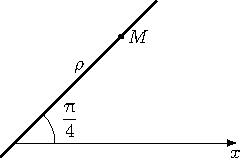
\includegraphics{4-15.pdf}
    \caption{}\label{fig:4-15}
  \end{figurehere}
\end{minipage}
\begin{equation}
  \label{eq:const_angle}
  \theta=\frac{\uppi}{4}.
\end{equation}

这就是所求的射线的极坐标方程。
方程中不含 $\rho$,说明射线上点的极坐标中的 $\rho$,无论取任何正值,$\theta$ 的对应值都是 $\dfrac{\uppi}{4}$。
\medskip
如果允许 $\rho$ 取负值时,\cref{eq:const_angle} 所表示的是倾斜角为 $\dfrac{\uppi}{4}$ 的一条直线。
如果 $\rho$ 不允许取负值,这条直线就要用两个方程 $\theta=\dfrac{\uppi}{4}$ 和 $\theta=\dfrac{5\uppi}{4}$ 来表示。



\begin{example}\label{exam:circle_rho_theta}
  求圆心是 $C\,(a,0)$,半径是 $a$ 的圆的极坐标方程。
\end{example}
\noindent
\begin{minipage}{0.6\linewidth}\parindent2em
\begin{solution}
  由已知条件,圆心在极轴上,圆经过极点 $O$。设圆和极轴的另一个交点是 $A$(\cref{fig:4-16}),那么 $OA=2a$。

  设 $M\,(\rho,\theta)$ 是圆上任意一点,则 $OM\perp AM$,可得
  \[|OM|=|OA|\cos\theta.\]

  
\end{solution}
\end{minipage}\hfill
\begin{minipage}{0.35\linewidth}
\begin{figurehere}
  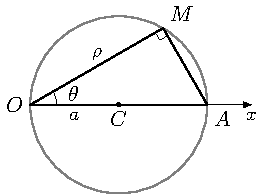
\includegraphics{4-16.pdf}
  \caption{}\label{fig:4-16}
\end{figurehere}
\end{minipage}

\medskip
用极坐标表示已知条件可得方程
\[\rho=2a\cos\theta.\]

这就是所求的圆的极坐标方程。

\begin{Practice}
  \begin{question}
    \item 求适合下列条件的直线的极坐标方程:
    \begin{tasks}(2)
      \task 过极点,倾斜角是 $\dfrac{\uppi}{6}$;
      \task 过点 $A\,(8,0)$,并且和极轴垂直。
    \end{tasks}
    \item 求适合下列条件的圆的极坐标方程:
    \begin{tasks}(2)
      \task 圆心在极点,半径为 3;
      \task 圆心在点 $A\,\left( {a,\dfrac{\uppi}{2}}\right)$,半径为 $a$。
    \end{tasks}
  \end{question}
\end{Practice}

\subsubsection{三种圆锥曲线的统一的极坐标方程}
在\cref{chp:conic_section}里我们曾经讲过,椭圆、双曲线、抛物线可以统一定义为: 与一个定点(焦点)的距离和一条定直线(准线)的距离的比等于常数 $e$ 的点的轨迹,当 $0<e<1$ 时是椭圆;$e>1$ 是双曲线;$e=1$ 是抛物线。
现在我们根据这个定义来求这三种圆锥曲线统一的极坐标方程。

过点 $F$ 作准线 $l$ 的垂线,垂足为 $K$,以焦点 $F$ 为极点,$FK$ 的反向延长线 $Fx$ 为极轴,建立极坐标系(\cref{fig:4-17})。

设 $M\,(\rho,\theta)$ 是曲线上任意一点,连结 $MF$,作 $MA \perp l$,$MB \perp Fx$ ,垂足分别为 $A$、$B$。那么曲线就是集合
\[P=\left\{M \middle\vert \frac{|MF|}{|MA|}=e \right\}.\]

\medskip\noindent
\begin{minipage}{0.65\linewidth}\parindent2em
  设焦点 $F$ 到准线 $l$ 的距离 $FK=p$。由 $|MF|=\rho$,$|MA|=|BK|=p+\rho\cos\theta$,得
  \[\frac{\rho}{p+\rho\cos\theta}=e,\]
  即
  \[\rho=\frac{ep}{1-e\cos\theta}.\]
\end{minipage}\hfill
\begin{minipage}{0.3\linewidth}
  \begin{figurehere}
    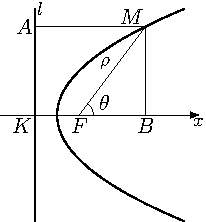
\includegraphics{4-17.pdf}
    \caption{}\label{fig:4-17}
  \end{figurehere}
\end{minipage}

\medskip
这就是椭圆、双曲线、抛物线的统一的极坐标方程。
当 $0<e<1$ 时,方程表示椭圆,定点 $F$ 是它的左焦点,定直线 $l$ 是它的左准线。
$e=1$ 时,方程表示开口向右的抛物线;$e>1$ 时,方程只表示双曲线右支,定点 $F$ 是它的右焦点,定直线 $l$ 是它的右准线,如果允许 $\rho< 0$,方程就表示整个双曲线(\cref{fig:4-18})。
\begin{figure}
  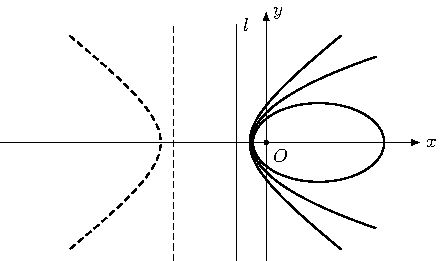
\includegraphics{4-18.pdf}
  \caption{}\label{fig:4-18}
\end{figure}

\begin{Practice}
  \begin{question}
    \item 以圆锥曲线的焦点为极点,焦点到准线的垂线的反向延长线为极轴,写出下列圆锥曲线的极坐标方程:
    \begin{tasks}
      \task 焦点到准线的距离是 5,离心率等于 2;
      \task 焦点到准线的距离是 3,离心率等于 $\dfrac{2}{3}$;
      \task 焦点到准线的距离是 4.5,离心率等于 1。
    \end{tasks}
    \item 判定下列圆锥曲线的极坐标方程表示什么曲线,再画出图形:
    \begin{tasks}(3)
      \task $\rho=\dfrac{4}{1-2\cos\theta}$;
      \task $\rho=\dfrac{4}{2-\cos\theta}$;
      \task $\rho=\dfrac{4}{2-2\cos\theta}$。
    \end{tasks}
  \end{question}
\end{Practice}

\subsection{极坐标方程和直角坐标的互化}
极坐标系和直角坐标系是两种不同的坐标系。
同一个点可以有极坐标,也可以有直角坐标;同一条曲线可以有极坐标方程,也可以有直角坐标方程。
为了研究问题方便,有时需要把在一种坐标系中的方程化为在另一种坐标系中的方程。

\medskip\noindent
\begin{minipage}{0.65\linewidth}\parindent2em
如\cref{fig:4-19},把直角坐标系的原点作为极点,$x$ 轴的正半轴作为极轴,并在两种坐标系中取相同的长度单位。
设 $M$ 是平面内任意一点,它的直角坐标是 $(x,y)$,极坐标是 $(\rho,\theta)$。从点 $M$ 作 $MN\perp Ox$,由三角函数定义,可以得出 $x$、$y$ 与 $\rho$、$\theta$ 之间的关系:
\end{minipage}\hfill
\begin{minipage}{0.3\linewidth}
  \begin{figurehere}
    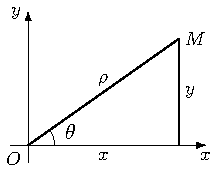
\includegraphics{4-19.pdf}
    \caption{}\label{fig:4-19}
  \end{figurehere}
\end{minipage}

\begin{equation}
  \label{eq:xy_vs_rhotheta}
  \tcbhighmath{x=\rho\cos\theta,\quad y=\rho\sin\theta}.
\end{equation}

由\cref{eq:xy_vs_rhotheta},可以得出下面的关系式:
\begin{equation}
  \label{eq:rhotheta_vs_xy}
  \tcbhighmath{\rho^2=x^2+y^2,\quad \tan\theta=\frac{y}{x}\,(x\neq 0)}.
\end{equation}

在一般情况下,由 $\tan\theta$ 确定角 $\theta$ 时,可根据点 $M$ 所在的象限取最小正角。

\begin{example}
  把点 $M$ 的极坐标 $\left(-5,\dfrac{\uppi}{6}\right)$ 化成直角坐标。
\end{example}
\begin{solution}
  \begin{align*}
  x&=-5\cos\dfrac{\uppi}{6}=-\dfrac{5}{2}\sqrt{3},\\
  y&=-5\sin\dfrac{\uppi}{6}=-\dfrac{5}{2}.
  \end{align*}
  
  $\therefore\quad$ 点 $M$ 的直角坐标是 $\left(-\dfrac{5}{2}\sqrt{3},-\dfrac{5}{2}\right)$。
\end{solution}

\begin{example}
  把点 $M$ 的直角坐标 $(-\sqrt{3},-1)$ 化成极坐标。
\end{example}
\begin{solution}
  \begin{gather*}
    \rho = \sqrt{(-\sqrt{3})^2+(-1)^2}=\sqrt{3+1}=2,\\
    \tan\theta=\frac{-1}{-\sqrt{3}}=\frac{1}{\sqrt{3}}.
  \end{gather*}
  
  $\because\quad$ 点 $M$ 在第三象限,$\rho>0$,$\therefore$ 最小正角 $\theta= \dfrac{7\uppi}{6}$。

  因此,点 $M$ 的极坐标是 $(2,\dfrac{7}{6}\uppi)$。
\end{solution}

\begin{example}
  化圆的直角坐标方程 $x^2+y^2-2ax=0$ 为极坐标方程。
\end{example}
\begin{solution}
  将\cref{eq:xy_vs_rhotheta} 代入原方程,得
  \[\rho^2\cos^2\theta+\rho^2\sin^2\theta-2a\rho\cos\theta=0,\]
  就是
  \[\rho=2a\cos\theta.\]
  当 $a>0$ 时,这个方程和\cref{subsec:polar_equation}\cref{exam:circle_rho_theta} 圆的极坐标方程相同。
\end{solution}

\begin{example}
  化圆锥曲线的极坐标方程 $\rho=\dfrac{ep}{1-e\cos\theta}$ 为直角坐标方程。
\end{example}
\begin{solution}
  原方程化为 $\rho=e\rho\cos\theta+ep$。

  将 $\rho\cos\theta=x$,$\rho=\sqrt{x^2+y^2}$ 代入上式,得 $\sqrt{x^2+y^2}= e(x+p)$,两边平方后,整理得
  \[ (1-e)x^2+y^2- 2e^2px-e^2p^2=0.\]

  这就是所求的直角坐标方程。
  但是,在将 $\sqrt{x^2+y^2}=e(x+p)$ 两边平方时,对于 $e>1$ 的情形,方程产生增根,这时方程表示整个双曲线,它相当于原极坐标方程允许 $\rho<0$ 的情形。
\end{solution}

\begin{Practice}
  \begin{question}
    \item 已知各点的极坐标为 $\left(4,\dfrac{\uppi}{4}\right)$、$\left( 2,\dfrac{4\uppi}{3}\right)$、$(-7,\uppi)$、$\left(5,\dfrac{\uppi}{2}\right)$、$\left(-2,-\dfrac{\uppi}{6}\right)$,求它们的直角坐标。
    \item 已知各点的直角坐标为 $(-1,-1)$、$(4,-4\sqrt{3})$、$(-3,4)$、$(0,-4)$,求它们的极坐标。
    \item 把下列直角坐标方程化成极坐标方程:
    \begin{tasks}(4)
      \task $x=5$;
      \task $y+4=0$;
      \task $2x-5y=0$;
      \task $x^2+y^2=25$。
    \end{tasks}
    \item 把下列极坐标方程化成直角坐标方程:
    \begin{tasks}(2)
      \task $\rho=7$;
      \task $\theta=\dfrac{\uppi}{4}$($\rho$ 可取负值);
      \task $\rho=4\cos\theta$;
      \task $\rho^2\cos2\theta=16$。
    \end{tasks}
  \end{question}
\end{Practice}

\subsection{等速螺线}
\medskip\noindent
\begin{minipage}{0.65\linewidth}\parindent2em
在机械传动中,常常需要把旋转运动变成直线运动。
\cref{fig:4-20} 中的凸轮装置就是借助凸轮绕定轴旋转推动从动杆作上、下往复直线运动。
在设计中,根据对从动杆运动的要求不同,需要设计不同的凸轮轮廓线。
如果需要从动杆作等速运动,凸轮的轮廓线就要用等速螺线。
\end{minipage}\hfill
\begin{minipage}{0.3\linewidth}
  \begin{figurehere}
    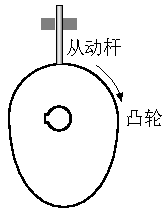
\includegraphics{4-20.pdf}
    \caption{}\label{fig:4-20}
  \end{figurehere}
\end{minipage}

\medskip\noindent
\begin{minipage}{0.65\linewidth}\parindent2em
什么是等速螺线呢? 如\cref{fig:4-21},从点 $O$ 出发的射线 $l$,绕点 $O$ 作等角速度的转动,同时点 $M$ 沿 $l$ 作等速直线运动,点 $M$ 的轨迹叫做\Concept{等速螺线}或\Concept{阿基米德螺线}。
\end{minipage}\hfill
\begin{minipage}{0.3\linewidth}
\begin{figurehere}
  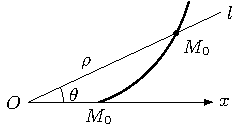
\includegraphics{4-21.pdf}
  \caption{}\label{fig:4-21}
\end{figurehere}
\end{minipage}

\medskip
下面,我们来求等速螺线的极坐标方程。

取点 $O$ 为极点,以 $l$ 的初始位置为极轴,建立极坐标系(\cref{fig:4-21})。

设 $M_0\,(\rho_0,0)$ 是点 $M$ 的初始位置,$M$ 在 $l$ 上运动的速度为 $v$,$l$ 绕点 $O$ 转动的角速度为 $\omega$,经过时间 $t$ 后,$l$ 旋转了 $\theta$ 角,点 $M$ 到达位置 $(\rho,\theta)$。根据等速螺线的定义,得
\[ \rho-\rho_0=vt,\quad \theta=\omega t.\]

这是以时间 $t$ 为参数的极坐标参数方程。消去参数 $t$ ,得
\[ \rho-\rho_0=\frac{v}{\omega}\theta. \]
这就是所求的等速螺线的极坐标方程。

设 $\dfrac{v}{\omega}=a$($a\neq 0$),得
\[\rho=\rho_0+a\theta.\]
这是等速螺线的极坐标方程的一般形式,$\rho$ 是 $\theta$ 的一次函数。

在特殊情况下,当 $\rho_0=0$ 时,等速螺线的方程变为
\[\rho=a\theta.\]
这时方程中的 $\rho$ 和 $\theta$ 成正比例。

\begin{example}
  画出等速螺线 $\rho=a\theta$($a>0$)的图形。
\end{example}
\begin{solution}
和直角坐标系中的画图步骤一样,给出 $\theta$ 的一系列允许值,算出 $\rho$ 的对应值,再根据对应值表,描点画图。
\begin{table}
  \begin{tblr}{colspec={*{11}{X[c]}},vline{2}={0.8pt},rowsep=5pt}
    $\theta$ & 0 & $\dfrac{\uppi}{4}$  & $\dfrac{\uppi}{2}$ & $\dfrac{3\uppi}{4}$ & $\uppi$ & $\dfrac{5\uppi}{4}$ & $\dfrac{3\uppi}{2}$ & $\dfrac{7\uppi}{4}$ & $2\uppi$ & $\cdots$\\
    $\rho$ & 0 & $\dfrac{\uppi}{4}a$  & $\dfrac{\uppi}{2}a$& $\dfrac{3\uppi}{4}a$ & $\uppi a$ & $\dfrac{5\uppi}{4}a$ & $\dfrac{3\uppi}{2}a$ & $\dfrac{7\uppi}{4}a$ & $2\uppi a$ & $\cdots$\\
  \end{tblr}
\end{table}

在 $\theta=\dfrac{\uppi}{4}$ 的射线上,截取 $|OA|=\dfrac{\uppi}{4}a$,得到点 $A$;在 $\theta=\dfrac{\uppi}{2}$ 的射线上,截取 $|OB|=\dfrac{\uppi}{2}a=2\cdot \dfrac{\uppi}{4}a$,得到点 $B$;用同样方法可得到点 $C$、$D$、……将这些点连成平滑的曲线,就是 $\rho={a\theta }$ 的图形(\cref{fig:4-22})。

如果 $\rho$ 允许取负值,当 $\rho$、$\theta$ 是方程 $\rho=a\theta$ 的解时,$-\rho$、$-\theta$ 也是方程的解。
因为以 $(\rho,\theta)$ 和 $(-\rho,-\theta)$ 为坐标的点,关于过极点垂直于极轴的直线对称,所以 $\rho=a\theta$ 的图形也关于该直线对称。
\cref{fig:4-22} 中的实线表示 $\rho$、$\theta$ 取正值时的螺线部分,虚线表示 $\rho$、$\theta$ 取负值时的螺线部分。
\end{solution}
\begin{figure}
  \begin{minipage}[b]{0.55\linewidth}\centering
    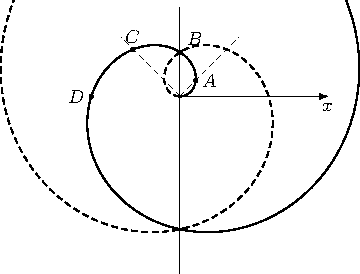
\includegraphics{4-22.pdf}
    \caption{}\label{fig:4-22}
  \end{minipage}
  \begin{minipage}[b]{0.4\linewidth}\centering
    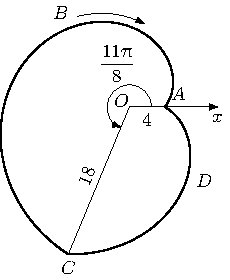
\includegraphics{4-23.pdf}
    \caption{}\label{fig:4-23}
  \end{minipage}
\end{figure}
\begin{example}
  \label{exp:cam}由于某种需要,设计一个凸轮,轮廓线如\cref{fig:4-23}。要求如下:

  凸轮依顺时针方向绕点 $O$ 转动,开始时从动杆接触点为 $A$,$|OA|=\qty{4}{cm}$。
  \begin{enumerate}
    \item 当从动杆接触轮廓线 $ABC$ 时,它被推向右方作等速直线运动。
    凸轮旋转角度 $\dfrac{11}{8}\uppi$ 时,有最大推程 \qty{14}{cm} 即 $|OC|=\qty{18}{cm}$;
    \item 当从动杆接触轮廓线 $CDA$ 时,它向左等速退回原位。
  \end{enumerate}
  求曲线 $ABC$ 及曲线 $CDA$ 的方程。
\end{example}

\begin{solution}
  取极坐标系,如\cref{fig:4-23}。

  由于曲线 $ABC$ 是等速螺线,设它的极坐标方程为
  \begin{equation}
    \label{eq:spiral_polar}
    \rho = \rho_0+a\theta.
  \end{equation}
  
  因为点 $A\,(4,0)$ 和点 $C\,\left(18,\dfrac{11}{8}\uppi\right)$ 都在曲线上,所以
  \[\begin{cases}4=\rho_0,\\18=\rho_0+a\cdot\dfrac{11}{8}\uppi.\end{cases}\]
  解这个方程组,得
  \[\rho_0=4,\quad a=\frac{112}{11\uppi}.\]
  代入\cref{eq:spiral_polar},得到曲线 $ABC$ 的极坐标方程为
  \[\rho=4+\frac{112}{11\uppi}\theta \left(0\leqslant\theta\leqslant\frac{11}{8}\uppi\right).\]
  
  同样,由于曲线 $CDA$ 也是等速螺线,设它的极坐标方程为
  \begin{equation}
    \label{eq:spiral_polar_2}
    \rho = \rho_1+a_1\theta.
  \end{equation}
  因为点 $C\,\left(18,\dfrac{11}{8}\uppi\right)$ 和点 $A\,(4,2\uppi)$ 都在曲线上,所以
  \[\begin{cases}18=\rho_1+a_1\cdot\dfrac{11\uppi}{8},\\4=\rho_1+a_1\cdot 2\uppi.\end{cases}\]
  解这个方程组,得
  \[\rho_1=44.8,\quad a_1=\frac{22.4}{\uppi}.\]
  因此,$CDA$ 这段曲线的极坐标方程是
  \[rho=48.8-\frac{22.4}{\uppi}\theta \left(\frac{11}{8}\uppi\leqslant\theta \leqslant 2\uppi\right).\]
\end{solution}

\begin{Practice}
  \begin{question}
    \item 如果 $M_1\,(\rho_1,\theta_1)$、$M_2\,(\rho_2,\theta_2)$ 是等速螺线上的两点,那么 $\rho_2-\rho_1$ 与 $\theta_2-\theta_1$ 成正比例。
    \item\label{prac:4-9-2} 
    某自动机床上有一个凸轮,它的轮廓线 $ACB$ 是一段等速螺线(如图),$A$ 点到旋转中心 $O$ 的距离 $\rho_0= \qty{60}{mm}$,轴心角 $\angle AOB= \ang{30}$,工作时曲线 $ACB$ 能把从动杆推出 \qty{5}{mm}。求这段等速螺线的极坐标方程。
    \begin{figurehere}
      \begin{minipage}{\linewidth}\centering
        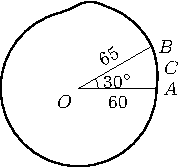
\includegraphics{pr4-9-2.pdf}
        \caption*{(第 \ref{prac:4-9-2} 题)}
      \end{minipage}
    \end{figurehere}
    \item 当 $0\geqslant\theta\geqslant-\dfrac{5\uppi}{8}$ 时,求本节\cref{exp:cam} 中的曲线 $ADC$ 的方程。
  \end{question}
\end{Practice}

\begin{Exercise}
  \begin{question}
    \item 已知 $A\,(\rho,\theta)$、$B\,(\rho,-\theta)$、$C\,(-\rho,-\theta)$、$D\,(-\rho,\theta)$,点 $A$ 和 $B$、$C$、$D$ 分别有怎样的相互位置关系?
    \item 说明下列极坐标方程表示什么曲线,并画图。
    \begin{tasks}(2)
      \task $\rho=3$;
      \task $\theta=\dfrac{\uppi}{3}$。
    \end{tasks}
    \item 求下列各图形的极坐标方程:
    \begin{tasks}
      \task 经过点 $A\,(3,\dfrac{\uppi}{3})$,平行于极轴的直线;
      \task 经过点 $A\,(-2,\dfrac{\uppi}{4})$,垂直于极轴的直线;
      \task 圆心在点 $A\,(5,\uppi)$,半径等于 5 的圆;
      \task 经过点 $A\,(a,0)$ 和极轴相交成 $\alpha$ 角的直线。
    \end{tasks}
    \item 画出下列极坐标方程的图形:
    \begin{tasks}(2)
      \task $\rho\cos\theta=2$;
      \task $\rho=6\cos\theta$;
      \task $\rho=10\sin\theta$;
      \task $\rho=10(1+\cos\theta)$。
    \end{tasks}
    \item 从极点作圆 $\rho=2a\cos\theta$ 的弦,求各个弦的中点的轨迹方程。
    \item 从极点 $O$ 作直线和直线 $\rho\cos\theta=4$ 相交于点 $M$,在 $OM$ 上取一点 $P$,使 $OM\cdot OP=12$,求 $P$ 点的轨迹的方程,并且说明轨迹是什么曲线。
    \item 一颗彗星的轨道是抛物线,太阳位于这条抛物线的焦点上。已知这颗彗星距太阳 \qty{1.6e8}{km} 时,极径和轨道的轴成 $\dfrac{\uppi}{3}$ 角。求这颗彗星轨道的极坐标方程,并且求它的近日点离太阳的距离。
    \item 把下列直角坐标方程化成极坐标方程:
    \begin{tasks}(2)
      \task $x^2+y^2=16$;
      \task $xy=a$;
      \task $x^2+y^2+2y=0$;
      \task $x^2-y^2=a^2$。
    \end{tasks}
    \item 把下列极坐标方程化成直角坐标方程:
    \begin{tasks}(2)
      \task $\rho=5\tan\theta$;
      \task $\rho+6\cot\theta\cdot\csc\theta=0$;
      \task $\rho=\dfrac{5}{\cos\theta}$;
      \task $\rho=\dfrac{6}{1-2\cos\theta}$;
      \task $\rho(2\cos\theta-5\sin\theta)-3=0$。
    \end{tasks}
    \item 已知一个圆的方程是 $\rho=5\sqrt{3}\cos\theta-5\sin\theta$,求圆心和半径。
    \item 长为 $2a$ 的线段,其端点在两个直角坐标轴上滑动,从原点作这条线段的垂线,垂足为 $M$,求点 $M$ 的轨迹的极坐标方程($Ox$ 为极轴),再化为直角坐标方程。
    \item\label{exec:14-12} 一凸轮如图所示,当它按箭头方向等速转动时,要求:
    \begin{tasks}
      \task 从动杆接触 $ABC$ 时,从动杆不动;
      \task 从动杆接触 $CDE$ 时,从动杆等速向右移动。
    \end{tasks}
    试按图中尺寸写出该凸轮轮廓线 $ABC$ 和 $CDE$ 的极坐标方程。
    \begin{figurehere}
      \begin{minipage}{\linewidth}\centering
        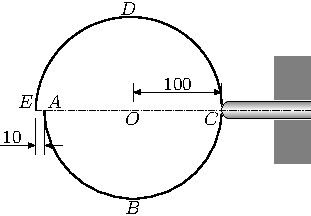
\includegraphics{ex14-12.pdf}
        \caption*{(第 \ref{exec:14-12} 题)}
      \end{minipage}
    \end{figurehere}
  \end{question}
\end{Exercise}

\section*{小结}
\begin{enumerate}[C、,itemindent=4.5em]
  \item 本章的主要内容是曲线的参数方程、极坐标系和曲线的极坐标方程,以及应用的初步知识。要注意,不仅在直角坐标系里可建立曲线的参数方程,在极坐标系里同样可以建立曲线的参数方程,不过这时是通过某个参数来表示 $\rho$ 和 $\theta$ 的关系。
  \item 在实际问题中,当我们求轨迹方程时,有时很难或不能找到曲线上点的坐标之间的直接关系。如果引进适当的参数,问题往往比较容易解决。研究运动的物体的轨迹时,常用时间作参数;研究旋转的物体的轨迹时,常用转角作参数。
  \item 化参数方程为普通方程的关键在于消去参数。反之,选择适当的参数也可以将普通方程化为参数方程。
  \item 和直角坐标系一样,极坐标系也是常用的一种坐标系。利用极坐标方程表示一些环绕一点作旋转运动的点的轨迹,比较方便。
  \item 极坐标和直角坐标可以互化。当把直角坐标系的原点作为极点,$x$ 轴的正半轴作为极轴时,点 $M$ 的直角坐标 $(x,y)$ 和极坐标 $(\rho,\theta)$ 有下面的关系:
  \[\begin{cases} x=\rho\cos\theta,\\y=\rho\sin\theta; \end{cases} \quad \begin{cases} \rho^2=x^2+y^2,\\\tan\theta=\dfrac{y}{x}\,(x\neq 0). \end{cases} \]
\end{enumerate}
\chapter*{复习参考题\chinese{chapter}}
\section*{A 组}
\begin{question}
  \item 叙述曲线和曲线的参数方程
  \[ \begin{cases} x=\varphi(t),\\y=\psi(t)  \end{cases}\]
  之间的对应关系。
  \item 设 $t$ 和 $\theta$ 是参数,化下列各参数方程为普通方程,并且画出它们的图形:
  \begin{tasks}(2)
    \task $\begin{cases} x=t^2-2t,\\ y=t^2+2;\end{cases}$
    \task $\begin{cases} x=5\cos\theta+2,\\ y=2\sin\theta-3.\end{cases}$
  \end{tasks}
  \item 把下列各方程按照所给条件化成参数方程 ($t$、$\theta$ 是参数):
  \begin{tasks}
    \task $x^2+2xy+y^2+2x-2y=0, \quad x=t-t^2$;
    \task $17x^2-16xy+4y^2-34x+16y+13=0, \quad x=1+2\cos\theta$。
  \end{tasks}
  \item 用描点法画出下列参数方程所表示的图形:
  \begin{tasks}(2)
    \task $\begin{cases} x=3t-5,\\ y=t^3-t; \end{cases}$
    \task $\begin{cases} x=5\cos\phi,\\ y=3\sin\phi; \end{cases}$
    \task $\begin{cases} x=\cos^3t,\\ y=\sin^3t; \end{cases}$
    \task $\begin{cases} x=t-\sin t,\\ y=1-\cos t. \end{cases}$
  \end{tasks}
  \item 已知弹道曲线的参数方程为
  \[ \begin{cases} x=v_0t\cos\alpha,\\ y=v_0t\sin\alpha-\dfrac{1}{2}gt^2,\end{cases} \]
  \begin{tasks}
    \task 求炮弹从发射到落回地面所需的时间;
    \task 求炮弹到达的最大高度。
  \end{tasks}
  \item 解答:
  \begin{enumerate}[itemindent=2em]
    \item 在 $\rho=\dfrac{3}{\cos\theta}$ 的图形上,求有下列极角的各点的坐标:
    \begin{tasks}(4)
      \task $\dfrac{\uppi}{3}$;
      \task $-\dfrac{\uppi}{3}$;
      \task $0$;
      \task $\dfrac{\uppi}{6}$。
    \end{tasks}
    \item 在 $\rho=\dfrac{1}{\sin\theta}$ 的图形上,求有下列极径的各点的坐标:
    \begin{tasks}(3)
      \task $1$;
      \task $2$;
      \task $\sqrt{2}$。
    \end{tasks}
  \end{enumerate}
  \item 求下列曲线的交点坐标,并画图:
  \begin{tasks}(2)
    \task $ \rho=4\sin\theta,\quad \rho=2$;
    \task $ \rho=\dfrac{3}{2-\cos\theta},\quad \rho=2$。
  \end{tasks}
  \item 说明下列方程表示什么曲线,并且画图:
  \begin{tasks}(2)
    \task $\rho=\dfrac{5}{1-\cos\theta}$;
    \task $\rho=\dfrac{5}{3-4\cos\theta}$;
    \task $\rho=\dfrac{1}{2-\cos\theta}$。
  \end{tasks}
  \item 求适合下列条件的点的轨迹的极坐标方程,并且画出它们的图形:
  \begin{tasks}
    \task 极径和极角成正比例;
    \task 极径和极角成反比例。
  \end{tasks}
  \item $O$ 是极点,$Ox$ 是极轴,点 $M$ 的坐标是 $(\rho,\theta)$,把 $Ox$ 绕点 $O$ 旋转角度 $\alpha$ 以后,$Ox$ 转到 $Ox'$ 的位置,对于新的极坐标系,点 $M$ 的坐标是 $(\rho',\theta')$,求点 $M$ 的新旧坐标之间的关系。
  \item 说明下列两条直线的位置关系:
  \begin{tasks}(2)
    \task $\theta=\alpha$ 和 $\rho\cos(\theta-\alpha)=\alpha$;
    \task $\theta=\alpha$ 和 $\rho\sin(\theta-\alpha)=a$。
  \end{tasks}
  \item 把下列各直角坐标方程化成极坐标方程:
  \begin{tasks}(2)
    \task $\left(x^2+y^2\right)^2=a^2\left(x^2-y^2\right)$;
    \task $x\cos\alpha+y\sin\alpha-p=0$;
    \task $x^2=2p\left(y+\dfrac{p}{2}\right)$。
  \end{tasks}
  \item 把下列极坐标方程化成直角坐标方程:
  \begin{tasks}(2)
    \task $\rho=64\sin^2\theta$;
    \task $\rho=-4\sin\theta+\cos\theta$;
    \task $\rho\cos\left(\theta-\dfrac{\uppi}{3}\right)=1$。
  \end{tasks}
  \item 等速螺线过点 $O\,(0,0)$ ,极角每增加 $\dfrac{\uppi}{3}$ 弧度,极径就增加 1.5。
  \begin{tasks}
    \task 求螺线的极坐标方程;
    \task 算出 $\theta=0,\ \dfrac{\uppi}{3},\ \dfrac{2\uppi}{3},\ \uppi,\ \dfrac{4\uppi}{3},\ \dfrac{5\uppi}{3},\ 2\uppi$ 所对应的 $\rho$ 的值;
    \task 描出上述各点,并作出 $0\leqslant \theta \leqslant 2\uppi$ 范围内螺线的图形。
  \end{tasks}
\end{question}
\section*{B 组}
\begin{question}[resume]
  \item \label{exec:4t-15} 如图,$OB$ 是机器上的曲柄,长是 $r$,绕点 $O$ 转动,$AB$ 是连杆,$M$ 是 $AB$ 上一点,$MA=a$,$MB=b$。当点 $A$ 在 $Ox$ 上作往返运动,点 $B$ 绕着点 $O$ 作圆运动时,求点 $M$ 的轨迹的参数方程。
  \begin{figure}
    \begin{minipage}{0.48\linewidth}\centering
      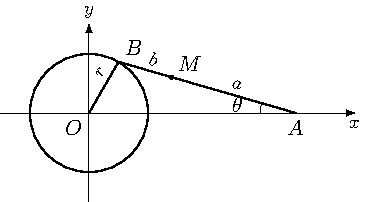
\includegraphics{4t-15.pdf}
      \caption*{(第 \ref{exec:4t-15} 题)}
    \end{minipage}
    \begin{minipage}{0.48\linewidth}\centering
      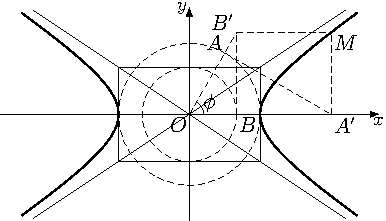
\includegraphics{4t-16.pdf}
      \caption*{(第 \ref{exec:4t-16} 题)}
    \end{minipage}
  \end{figure}
  \item \label{exec:4t-16}根据双曲线 $\dfrac{x^2}{a^2}-\dfrac{y^2}{b^2}=1$ 的图中所给出的 $\phi$,说明它的参数方程是
  \[\begin{cases} x=a\sec\phi,\\ y=b\tan\phi.\end{cases} \]
  并研究根据不同的 $\phi$,如何作出双曲线的一些点来画双曲线(图中的大圆半径是 $a$,小圆半径是 $b$)。
  \item 从圆周上定点 $O$ 引直线 $OS$ ,交圆于 $Q$,在 $OS$ 上取点 $P$,使 $| QP|=b$(常数)。当 $OS$ 绕 $O$ 旋转时;点 $P$ 的轨迹称为帕斯卡蚶线。求它的极坐标方程。
\end{question}

\chapter*{总复习参考题}
\section*{A 组}
\begin{question}
  \item 已知直线 $3x+4y-10+\lambda(4x-6y+7)=0$ 通过点 $A\,(4,7)$,求 $\lambda$ 的值。
  \item 已知点 $P\,(2,0)$、$Q\,(8,0)$。点 $M$ 到点 $P$ 的距离是它到点 $Q$ 的距离的 $\dfrac{1}{5}$ ,求点 $M$ 的轨迹方程。
  \item 点 $M\,(x,y)$ 到两个定点 $M_1$、$M_2$ 距离的比是一个正数 $m$,求点 $M$ 的轨迹方程,并说明轨迹是什么图形(考虑 $m = 1$ 和 $m \neq 1$ 两种情形)。
  \item 求证:以 $A\,(4,1)$、$B\,(1,5)$、$C\,(-3,2)$、$D\,(0,-2)$ 为顶点的四边形是正方形。
  \item 求证:以 $A\,(-4,-2)$、$B\,(2,0)$、$C\,(8,6)$、$D\,(2,4)$ 为顶点的四边形是平行四边形。并求它两边的夹角。
  \item 已知: 四边形一组对边的平方和等于另一组对边的平方和。求证: 两条对角线互相垂直。
  \item 把函数 $y=f(x)$ 在 $x=a$ 及 $x=b$ 之间的一段图象近似地看作直线,设 $a\leqslant c\leqslant b$ ,证明 $f(c)$ 的近似值是
  \[ f(a)+\frac{c-a}{b-a}[f(b)-f(a)].\]
  \item 求证:过点 $P(a\cos^3\alpha,a\sin^3\alpha)$ 且与直线 $x\sec\alpha+y\csc\alpha=a$ 垂直的直线方程是 $x\cos\alpha-y\sin\alpha=a\cos2\alpha$。
  \item 判定两圆 $x^2+y^2-6x+4y+12=0$,$x^2+y^2-14x-2y+14=0$ 是否相切。
  \item 已知椭圆的方程是 $\frac{x^2}{16}+\frac{y^2}{9}=1$。求椭圆内接正方形的面积。
  \item 证明: 等轴双曲线上任意一点到中心的距离是它到两个焦点的距离的比例中项。
  \item 设抛物线的轴和它的准线相交于点 $A$,经过焦点垂直于轴的直线交抛物线于 $B$、$C$ 两点。求证:$BA\perp CA$。
  \item 把点 $A\,(a,b)$ 的坐标变成下列新坐标,求坐标轴旋转角的正弦或余弦值:
  \begin{tasks}(2)
    \task $(-a,-b)$;
    \task $(-a,b)$;
    \task $(a,-b)$;
    \task $(b,a)$。
  \end{tasks}
  \item 求曲线 $y^2=4-2x$ 上距离原点最近的点 $P$ 的坐标。
  \item 证明:$\sqrt{x}+\sqrt{y}=\sqrt{a}$($a>0$)是一段抛物线。求出它的顶点坐标和焦点坐标。
  \item 在直角坐标系中化简方程
  \[(1-e^2)x^2+y^2-2e^2px-e^2p^2=0\]
  当
  \begin{tasks}(3)
    \task $e<1$;
    \task $e>1$;
    \task $e=1$
  \end{tasks}
  时,求出它在原坐标系中的焦点坐标和准线方程。
  \item 把圆锥曲线的极坐标方程 $\rho=\dfrac{p}{2-\cos\theta}$ 化成直角坐标方程,再移轴化成标准方程。
  \item 定点 $M$ 的极坐标为 $(10,\ang{30})$,已知极点 $O'$ 在直角坐标系 $xOy$ 中的坐标为 $(2,3)$,极轴平行于 $x$ 轴,且极轴的正方向与 $x$ 轴的正方向相同,两个坐标系的长度单位也相同,求点 $M$ 的直角坐标。
  \item\label{exec:tt-19} 如图,设基圆半径为 $r$,渐开线的起点为 $A$,取圆心 $O$ 为极点,射线 $OA$ 为极轴。$M\,(\rho,\theta)$ 为渐开线上任一点,过 $M$ 作基圆的切线 $MB$,$B$ 是切点。设 $\angle BOM=\alpha$。试用 $\alpha$ 做参数,写出渐开线在极坐标系中的参数方程。
  \begin{figure}
    \begin{minipage}[b]{0.3\linewidth}\centering
      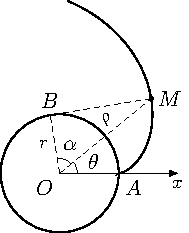
\includegraphics{tt-19.pdf}
      \caption*{(第 \ref{exec:tt-19} 题)}
    \end{minipage}%
    \begin{minipage}[b]{0.65\linewidth}\centering
      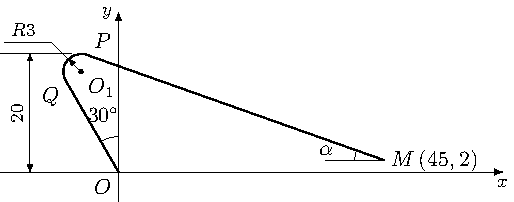
\includegraphics{tt-22.pdf}
      \caption*{(第 \ref{exec:tt-22} 题)}
    \end{minipage}
  \end{figure}
  \item 从极点 $O$ 引一条直线和圆 $\rho^2-2a\rho\cos\theta+ a^2-r^2=0$ 相交于一点 $Q$,点 $P$ 分线段 $\overline{OQ}$ 成比 $m:n$,求点 $Q$ 在圆上移动时,点 $P$ 的轨迹方程,并画出图形。
\end{question}
\section*{B 组}
\begin{question}[resume]
  \item 某生产大队科学试验小组,为了提高玉米的产量,在试验田进行追施硝氨肥的试验,得到如下数据:
  \par\noindent%
  \begin{tablehere}%
  \begin{tblr}{colspec={c*{8}{X[r]}},row{1}={m,c},vline{2}={0.8pt}}
    追肥量 $x$(\unit{kg})& 1 & 2 & 3 & 4 & 5 & 6 & 7 & 8 \\
      产量 $y$(\unit{kg})& 120 & 123 & 125 & 128.5 & 131 & 133.5 & 136 & 139 \\
  \end{tblr}
  \end{tablehere}
  用平均值法求这范围内的 $y$ 与 $x$ 之间的经验公式。
  \item \label{exec:tt-22}图中表示凸模的一部分外形曲线,线段 $OQ$、$MP$ 分别和圆弧 $\overparen{QP}$ 切于 $Q$、$P$ 两点,建立如图所示的坐标系,试根据图中数据,求圆心 $O_1$ 的坐标和 $\alpha$ 角的大小。
  \item 证明: $(A_1-C_1)B_2=(A_2-C_2)B_1\neq 0$ 时,二次曲线
  \begin{gather*}
    A_1x^2+B_1xy+C_1y^2+D_1x+E_1y+F_1=0,\\
    A_2x^2+B_2xy+C_2y^2+D_2x+E_2y+F_2=0
  \end{gather*}
  的交点在同一个圆上。
  \item 已知方程 $16x^2+ky^2=16k$,讨论当 $k$ 取不同数值时,它表示什么曲线?
  \item 直线 $y=x+b$ 与抛物线 $y=x^2-3x+5$ 相交于两点,求这两点连线的中点的轨迹方程。
  \item \label{exec:tt-26}一个半径是 $4r$ 的定圆 $O$ 和一个半径是 $r$ 的动圆 $C$ 相内切。当圆 $C$ 滚动时,求证圆 $C$ 上定点 $M$ (开始时在 $A$ 点)的轨迹的方程是
  \[\begin{cases} x=r(3\cos\phi+cos3\phi),\\y=r(3\sin\phi-\sin3\phi).  \end{cases}\]
  证明这个方程可以化成 
  \[ \begin{cases} x=4r\cos^3\phi,\\y=4r\sin^3\phi,\end{cases} \] 
  并且求出它的普通方程。
  \item \label{exec:tt-27}如图,$OA$ 是定圆的直径,它的长是 $2a$,直线 $OB$ 和圆相交于点 $M_1$,和经过点 $A$ 的切线相交于点 $B$。$MM_1\perp OA$,$MB\parallel OA$,$MM_1$ 与 $MB$ 相交于点 $M$。以点 $O$ 为原点,$OA$ 方向为 $x$ 轴的正向,求点 $M$ 的轨迹的参数方程(以 $\dot{\theta}$ 为参数)。
  \begin{figure}
    \begin{minipage}[b]{0.65\linewidth}\centering
      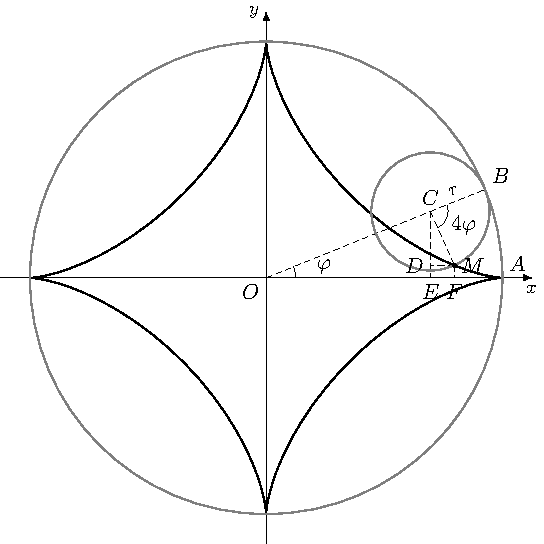
\includegraphics{tt-26.pdf}
      \caption*{(第 \ref{exec:tt-26} 题)}
    \end{minipage}
    \begin{minipage}[b]{0.3\linewidth}\centering
      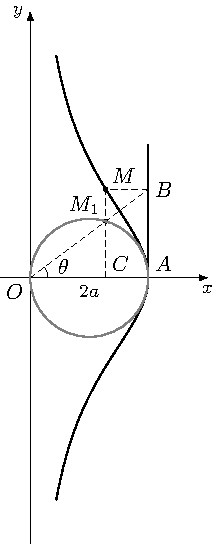
\includegraphics{tt-27.pdf}
      \caption*{(第 \ref{exec:tt-27} 题)}
    \end{minipage}
  \end{figure}
\end{question}